% ASSERT_CONVENTION: natural_units=natural, metric_signature=mostly_minus, fourier_convention=physics, coupling_convention=alpha_s, generator_normalization=T(fund)=1/2, covariant_derivative_sign=D_mu=partial_mu-igA
%
% Lecture 9: The Landscape of SUSY Dualities
% Part of: The Dualised Standard Model -- Part III Lecture Notes
%
% Conventions (Seiberg hep-th/9411149, unchanged from Lectures 1-8):
%   T(fund SU(N)) = 1/2 per Weyl fermion
%   b_0 = (11N_c - 2N_f)/3 for N_f Dirac flavours (SU case)
%   A(fund) = 1 (cubic anomaly coefficient per fundamental Weyl fermion)
%   alpha_s = g_s^2 / (4 pi)
%   R[Q] = (N_f - N_c)/N_f; R[W] = 2
%   N_f counts Dirac flavour pairs (each = 2 Weyl fermions) for SU
%
% NEW CONVENTIONS FOR THIS LECTURE (Intriligator-Seiberg):
%   Sp(N_c) = rank N_c, fundamental dimension 2N_c.  Sp(1) = SU(2).
%   SO(N_c) with N_c-dimensional vector representation
%   T(vector SO(N_c)) = 1 (NOT 1/2)
%   T(fund Sp(N_c)) = 1/2 (same normalisation as SU)
%   T(antisym_2 Sp(N_c)) = N_c - 1
%   Dual Coxeter numbers: h(SU(N)) = N, h(SO(N)) = N-2, h(Sp(N)) = N+1
%
\documentclass[11pt,a4paper]{article}
% ASSERT_CONVENTION: natural_units=natural, metric_signature=mostly_minus, fourier_convention=physics, coupling_convention=alpha_s, generator_normalization=T(fund)=1/2, covariant_derivative_sign=D_mu=partial_mu-igA
%
% CONVENTIONS (Seiberg hep-th/9411149)
% Metric: (+,-,-,-) (mostly minus)
% T(fund) = 1/2 per Weyl fermion
% b_0 = (11N_c - 2N_f)/3 for N_f Dirac flavours
% D_mu = partial_mu - ig A_mu^a T^a
% A(fund) = 1 (cubic anomaly coefficient per fundamental Weyl fermion)
% alpha_s = g_s^2 / (4 pi)
% R[Q] = (N_f - N_c)/N_f; R[W] = 2
% N_f counts Dirac flavour pairs (each = 2 Weyl fermions)
%
% This file is \input{} by all lecture files.

%% ---------- Document class ----------
% (loaded by the wrapper; preamble only provides packages and macros)

%% ---------- Standard packages ----------
\usepackage{amsmath,amssymb,amsthm,mathtools}
\usepackage{hyperref}
\usepackage[capitalise,noabbrev]{cleveref}
\usepackage{enumitem}
\usepackage{booktabs}
\usepackage{array}
\usepackage{xcolor}
\usepackage{tikz}
\usetikzlibrary{arrows.meta,decorations.markings,positioning,calc}
\usepackage{fancybox}
\usepackage{tcolorbox}
\tcbuselibrary{skins,breakable}
\usepackage{slashed}              % Feynman slash notation
\usepackage{cite}                 % compressed citation lists

%% ---------- Hyperref configuration ----------
\hypersetup{
  colorlinks=true,
  linkcolor=blue!70!black,
  citecolor=green!50!black,
  urlcolor=blue!80!black,
  pdfauthor={Part III Lecture Notes},
  pdftitle={The Dualised Standard Model}
}

%% ---------- Theorem environments ----------
\theoremstyle{plain}
\newtheorem{theorem}{Theorem}[section]
\newtheorem{lemma}[theorem]{Lemma}
\newtheorem{proposition}[theorem]{Proposition}
\newtheorem{corollary}[theorem]{Corollary}

\theoremstyle{definition}
\newtheorem{definition}[theorem]{Definition}
\newtheorem{example}[theorem]{Example}
\newtheorem{exercise}{Exercise}[section]

\theoremstyle{remark}
\newtheorem{remark}[theorem]{Remark}

%% ---------- Physics macros: gauge groups and representations ----------
\newcommand{\Nc}{N_{\!c}}
\newcommand{\Nf}{N_{\!f}}
\newcommand{\SU}[1]{\mathrm{SU}(#1)}
\newcommand{\UU}[1]{\mathrm{U}(#1)}

% Representations
\newcommand{\fund}{\square}
\newcommand{\antifund}{\overline{\square}}
\newcommand{\adj}{\mathrm{adj}}
\newcommand{\antisym}{\wedge^{\!2}}        % antisymmetric rank-2
\newcommand{\sym}{\mathrm{S}_2}           % symmetric rank-2

%% ---------- Physics macros: group theory constants ----------
% Dynkin index: Tr(T^a T^b) = T(R) delta^{ab}
\newcommand{\Tfund}{\tfrac{1}{2}}          % T(fund) = 1/2 per Weyl fermion
\newcommand{\Tadj}{\Nc}                    % T(adj) = N_c
\newcommand{\Cfund}{\frac{\Nc^2 - 1}{2\Nc}}  % C_2(fund)
\newcommand{\Cadj}{\Nc}                    % C_2(adj)

% Cubic anomaly coefficient: A(R) = Tr_R[T^a {T^b, T^c}] with A(fund) = 1
\newcommand{\Afund}{1}

%% ---------- Physics macros: beta function ----------
\newcommand{\bzero}{b_0}
\newcommand{\bone}{b_1}
\newcommand{\alphas}{\alpha_s}
\newcommand{\gs}{g_s}

%% ---------- Physics macros: SUSY / R-charge ----------
\newcommand{\Rcharge}[1]{R[#1]}
\newcommand{\Wsup}{W}                      % superpotential

%% ---------- Physics macros: covariant derivative and field strength ----------
\newcommand{\Dmu}{D_\mu}
\newcommand{\Fmn}{F_{\mu\nu}}
\newcommand{\Ftilde}{\widetilde{F}_{\mu\nu}}

%% ---------- Physics macros: common abbreviations ----------
\newcommand{\ie}{\textit{i.e.}}
\newcommand{\eg}{\textit{e.g.}}
\newcommand{\cf}{\textit{cf.}}
\newcommand{\IR}{\ensuremath{\mathrm{IR}}}
\newcommand{\UV}{\ensuremath{\mathrm{UV}}}
\newcommand{\AF}{\ensuremath{\mathrm{AF}}}
\newcommand{\BZ}{\ensuremath{\mathrm{BZ}}}
\newcommand{\NSVZ}{\ensuremath{\mathrm{NSVZ}}}
\newcommand{\SQCD}{\ensuremath{\mathrm{SQCD}}}
\newcommand{\QCD}{\ensuremath{\mathrm{QCD}}}
\newcommand{\SM}{\ensuremath{\mathrm{SM}}}
\newcommand{\Tr}{\mathrm{Tr}}

%% ---------- Convention box macro ----------
\newtcolorbox{conventionbox}[1][]{%
  enhanced,
  colback=blue!5!white,
  colframe=blue!60!black,
  fonttitle=\bfseries,
  title={Conventions},
  #1
}

%% ---------- Comparison table style ----------
\newtcolorbox{comparisontable}[1][]{%
  enhanced,
  colback=orange!5!white,
  colframe=orange!70!black,
  fonttitle=\bfseries,
  title={Comparison},
  #1
}

%% ---------- Warning / important box ----------
\newtcolorbox{warningbox}[1][]{%
  enhanced,
  colback=red!5!white,
  colframe=red!70!black,
  fonttitle=\bfseries,
  title={Important},
  #1
}

%% ---------- Preview / forward-reference box ----------
\newtcolorbox{previewbox}[1][]{%
  enhanced,
  colback=green!5!white,
  colframe=green!50!black,
  fonttitle=\bfseries,
  title={Preview},
  #1
}

%% ---------- Page layout ----------
\usepackage[margin=2.5cm]{geometry}
\setlength{\parskip}{0.4em}
\setlength{\parindent}{0em}

%% ---------- Section formatting ----------
\usepackage{titlesec}
\titleformat{\section}{\Large\bfseries}{\thesection}{1em}{}
\titleformat{\subsection}{\large\bfseries}{\thesubsection}{1em}{}

%% ---------- End of preamble ----------


%% ---------- Additional macros for this lecture ----------
\newcommand{\SO}[1]{\mathrm{SO}(#1)}
\newcommand{\Sp}[1]{\mathrm{Sp}(#1)}
\newcommand{\Nctilde}{\widetilde{N}_{\!c}}

\title{\textbf{Lecture 9: The Landscape of SUSY Dualities}}
\author{The Dualised Standard Model --- Part III Lecture Notes}
\date{Lent Term 2027}

\begin{document}
\maketitle

\tableofcontents
\newpage

%% ========================================================================
%%  CONVENTIONS
%% ========================================================================

\begin{conventionbox}[title={Conventions for Lecture 9}]
All conventions from Lectures~1--8 remain in force.  This lecture
introduces orthogonal and symplectic gauge groups, which require
additional index conventions.

\renewcommand{\arraystretch}{1.3}
\begin{tabular}{@{}l l l@{}}
\toprule
\textbf{Quantity} & \textbf{Convention} & \textbf{Comment} \\
\midrule
Units & $\hbar = c = 1$ (natural) & \\
Metric & $\eta_{\mu\nu} = \mathrm{diag}(+1,-1,-1,-1)$ & mostly minus \\
Dynkin index (SU) & $\Tr(T^a T^b) = \Tfund\, \delta^{ab}$ & fundamental of $\SU{\Nc}$ \\
Cubic anomaly & $A(\fund) = 1$, $A(\antifund) = -1$ & per fundamental Weyl \\
$\Nf$ counting (SU) & Dirac flavour pairs & each $= (Q_i, \widetilde{Q}_i)$ \\
\midrule
\multicolumn{3}{@{}l}{\textbf{New in this lecture:}} \\
$\SO{\Nc}$ convention & $\Nc$-dimensional vector representation & \\
$T(\text{vector } \SO{\Nc})$ & $1$ & \textbf{not} $\tfrac{1}{2}$; see~\cite{IS1995} \\
$\Sp{\Nc}$ convention & \textbf{rank} $\Nc$; fund.\ dim.\ $2\Nc$ & $\Sp{1} = \SU{2}$ \\
$T(\text{fund } \Sp{\Nc})$ & $\tfrac{1}{2}$ & same as SU \\
$T(\antisym\; \Sp{\Nc})$ & $\Nc - 1$ & antisymmetric of $\Sp{\Nc}$ \\
Dual Coxeter number & $h_{\SU{N}} = N$,\; $h_{\SO{N}} = N-2$,\; $h_{\Sp{N}} = N+1$ & \\
\bottomrule
\end{tabular}
\end{conventionbox}

\begin{warningbox}[title={The $\Sp{N}$ naming convention}]
The symplectic group is named inconsistently across the literature.
We follow \textbf{Intriligator and Seiberg}~\cite{IS9506101,IS1995}:
$\Sp{\Nc}$ denotes the group of \textbf{rank}~$\Nc$ whose
fundamental representation has dimension~$2\Nc$.
Thus $\Sp{1} = \SU{2}$ and $\Sp{2}$ has a $4$-dimensional
fundamental.  Some mathematics references write $\Sp{2\Nc}$ for the
same group (labelling by the dimension of the fundamental rather
than the rank).
\textbf{Verify:} $\Sp{1}$ has $\dim(\text{fund}) = 2$, matching
$\SU{2}$.\;\checkmark
\end{warningbox}


%% ========================================================================
%%  SECTION 1: Recap and Motivation
%% ========================================================================
\section{Recap and Motivation}
\label{sec:recap-motivation}

In Lecture~3, we established Seiberg duality~\cite{Seiberg1995} for
$\mathcal{N}=1$ $\SU{\Nc}$ SQCD with $\Nf$ fundamental flavours: the
IR physics of the electric theory is equivalently described by a
\emph{magnetic} $\SU{\Nf - \Nc}$ gauge theory with $\Nf$ dual quarks
and an elementary $\Nf \times \Nf$ meson matrix~$M$.
We verified this statement through six independent 't~Hooft anomaly
coefficients, mass deformation consistency, and moduli space matching.
The conformal window $\tfrac{3}{2}\Nc < \Nf < 3\Nc$ was identified as
the regime where both descriptions flow to the same IR fixed point.

A natural question arises: \emph{is Seiberg duality a peculiarity of
$\SU{\Nc}$ with fundamental matter, or does it extend to other gauge
groups and representations?}  The answer, developed through an
intensive programme in the mid-1990s, is that electric--magnetic
duality is a \emph{pervasive structural feature} of strongly coupled
$\mathcal{N}=1$ gauge theories.  Dualities have been established for:
\begin{itemize}
  \item $\SU{\Nc}$ with fundamental \emph{and adjoint} matter
    (Kutasov--Schwimmer~\cite{KS9505004});
  \item orthogonal gauge groups $\SO{\Nc}$
    (Intriligator--Seiberg~\cite{IS9506101});
  \item symplectic gauge groups $\Sp{\Nc}$
    (Intriligator--Seiberg~\cite{IS9506101});
  \item product gauge groups and quiver gauge theories;
  \item theories exhibiting \emph{s-confinement} without a dual gauge
    group (Cs\'aki--Schmaltz--Skiba~\cite{CSS9612207});
  \item cascading gauge theories in which repeated Seiberg dualities
    drive a renormalisation group flow
    (Klebanov--Strassler~\cite{KlebanovStrassler2000}).
\end{itemize}

This lecture surveys the established landscape of $\mathcal{N}=1$ SUSY
dualities, organised by gauge group (following the pedagogical approach
of Peskin~\cite{Peskin1997} and Intriligator--Seiberg~\cite{IS1995}).
The unifying thread is
\textbf{'t~Hooft anomaly matching}: in every case, the anomaly
coefficients of the global symmetry group match exactly between the
electric and magnetic descriptions.  We verify one anomaly coefficient
explicitly for each new gauge group, confirming that the general
framework extends consistently beyond $\SU{\Nc}$.

\begin{previewbox}[title={Connection to the dualised SM}]
The dualised Standard Model of Lectures~7--8 employs Seiberg duality
for an $\SU{N}$ electric theory with fundamental and adjoint matter
(the Pati--Salam embedding).  The Kutasov--Schwimmer duality of
\S\ref{sec:kutasov-schwimmer} is therefore the most directly relevant
generalisation for the dualised SM programme.  The SO and Sp dualities
demonstrate the \emph{breadth} of the duality phenomenon.
\end{previewbox}


%% ========================================================================
%%  SECTION 2: Kutasov-Schwimmer Duality
%% ========================================================================
\section{Kutasov--Schwimmer Duality: $\SU{\Nc}$ with Adjoint Matter}
\label{sec:kutasov-schwimmer}

\subsection{Electric theory}

Consider $\mathcal{N}=1$ $\SU{\Nc}$ with the following matter content:
\begin{itemize}
  \item $\Nf$ chiral superfields $Q^i$ in the fundamental ($\fund$)
    and $\Nf$ chiral superfields $\widetilde{Q}_i$ in the
    antifundamental ($\antifund$), where $i = 1, \ldots, \Nf$.
  \item One chiral superfield $\Phi$ in the adjoint representation
    ($\adj$).
  \item A tree-level superpotential:
    \begin{equation}\label{eq:KS-W-el}
      W_{\text{el}} = \frac{g}{k+1}\,\Tr\!\left(\Phi^{k+1}\right)\,,
    \end{equation}
    where $k \geq 1$ is a positive integer and $g$ is a coupling
    constant.
\end{itemize}

The superpotential~\eqref{eq:KS-W-el} is a relevant deformation
that lifts the flat directions associated with the adjoint field.
The integer~$k$ parametrises a \emph{family} of theories, each with
a different conformal window and a different dual description.

\subsection{The dual (magnetic) theory}
\label{ssec:ks-magnetic}

Kutasov and Schwimmer~\cite{KS9505004}, with further developments
by Kutasov, Schwimmer, and Seiberg~\cite{KSS9507040}, showed that
the IR physics of the electric theory is equivalently described by
the following \textbf{magnetic theory}:

\begin{tcolorbox}[
  enhanced,
  colback=blue!5!white,
  colframe=blue!70!black,
  fonttitle=\bfseries\large,
  title={Kutasov--Schwimmer Duality},
  breakable
]
\textbf{Electric:} $\SU{\Nc}$ with $\Nf \times (Q, \widetilde{Q})$
$+$ adjoint $\Phi$, \quad $W_{\text{el}} = \dfrac{g}{k+1}\,
\Tr(\Phi^{k+1})$.

\medskip

\textbf{Magnetic:}
\begin{itemize}
  \item \textbf{Gauge group:} $\SU{k\Nf - \Nc}$.
  \item \textbf{Dual quarks:} $\Nf$ chiral superfields $q_i$
    ($\fund$) and $\Nf$ chiral superfields $\widetilde{q}^{\,i}$
    ($\antifund$) of $\SU{k\Nf - \Nc}$.
  \item \textbf{Dual adjoint:} one chiral superfield $\phi$ in the
    adjoint of $\SU{k\Nf - \Nc}$.
  \item \textbf{Mesons:} $k$ gauge-singlet chiral superfields
    $M_j^{\ i}{}_{\!l}$ ($j = 0, 1, \ldots, k-1$), defined by the
    map from the electric theory:
    \begin{equation}\label{eq:KS-meson-map}
      M_j \;\sim\; Q\, \Phi^j\, \widetilde{Q}\,,
      \qquad j = 0, 1, \ldots, k-1\,.
    \end{equation}
    Each $M_j$ is an $\Nf \times \Nf$ matrix transforming as
    $(\fund, \antifund)$ under $\SU{\Nf}_L \times \SU{\Nf}_R$.
  \item \textbf{Magnetic superpotential:}
    \begin{equation}\label{eq:KS-W-mag}
      W_{\text{mag}} = \frac{g'}{k+1}\,\Tr(\phi^{k+1})
      + \sum_{j=0}^{k-1} \frac{1}{\mu_j}\,
      \Tr\!\left(M_j\, q\, \phi^{k-1-j}\, \widetilde{q}\right)\,.
    \end{equation}
\end{itemize}
\end{tcolorbox}

The key features distinguishing Kutasov--Schwimmer (KS) duality from
basic Seiberg duality are:
\begin{enumerate}
  \item The dual gauge group is $\SU{k\Nf - \Nc}$, with the
    integer~$k$ appearing as a \emph{multiplier} of $\Nf$.
  \item The dual theory retains an adjoint chiral superfield~$\phi$
    with the same polynomial superpotential.
  \item There are $k$ distinct meson species $M_0, M_1, \ldots,
    M_{k-1}$, arising from the electric operators
    $Q\Phi^j\widetilde{Q}$ for $j = 0, \ldots, k-1$.
    The operator $Q\Phi^k\widetilde{Q}$ and higher powers are
    related to lower ones via the equation of motion
    $\partial W_{\text{el}}/\partial \Phi = 0$, which gives the
    chiral ring relation $\Phi^k \sim 0$ (up to lower powers).
\end{enumerate}

\subsection{Conformal window}

Both the electric and magnetic theories must be asymptotically free
for the duality to produce a non-trivial interacting fixed point.
The one-loop beta function coefficient for $\SU{\Nc}$ with $\Nf$
fundamentals and one adjoint is:
\begin{equation}\label{eq:KS-beta}
  b_0^{\text{el}} = 3\Nc - \Nf - \Nc = 2\Nc - \Nf\,,
\end{equation}
using $T(\adj) = \Nc$ and $T(\fund) = \tfrac{1}{2}$.  (The factor
of $\Nc$ from the adjoint replaces $\Nc$ in the usual $3\Nc - \Nf$
by $3\Nc - \Nc = 2\Nc$, because the adjoint contributes as if it
were $\Nc$ additional flavours.)

However, the superpotential $W = \Tr(\Phi^{k+1})$ constrains the
anomalous dimension of $\Phi$ at the fixed point to
$\gamma_\Phi^* = -2/(k+1)$ (so that $W$ has $R$-charge~$2$).
Incorporating this constraint, the effective conformal window
becomes~\cite{KS9505004,KSS9507040}:
\begin{equation}\label{eq:KS-window}
  \boxed{\frac{3\Nc}{k+1} < \Nf < \frac{3\Nc}{k}}\,.
\end{equation}
The upper bound $\Nf < 3\Nc/k$ ensures $b_0^{\text{el}} > 0$
after accounting for the adjoint's anomalous dimension at the
fixed point; the lower bound ensures the same for the magnetic
theory.

\subsection{The $k=1$ limit: recovering Seiberg duality}
\label{ssec:KS-k1-limit}

The crucial consistency check is that the $k=1$ case reduces to the
Seiberg duality of Lecture~3.

\begin{tcolorbox}[
  enhanced,
  colback=green!5!white,
  colframe=green!60!black,
  fonttitle=\bfseries,
  title={KS at $k=1$: Recovering Seiberg Duality},
  breakable
]
\textbf{Step 1: Electric theory at $k=1$.}
The superpotential becomes
\[
  W_{\text{el}} = \frac{g}{2}\,\Tr(\Phi^2)\,.
\]
This is simply a \textbf{mass term} for the adjoint field $\Phi$.
In the IR (below the mass scale $m_\Phi = g$), we integrate out
$\Phi$, leaving pure $\SU{\Nc}$ SQCD with $\Nf$ fundamental
flavours and $W = 0$ --- exactly the electric theory of Lecture~3.

\medskip

\textbf{Step 2: Magnetic gauge group at $k=1$.}
\[
  \SU{k\Nf - \Nc}\big|_{k=1} = \SU{\Nf - \Nc}\,.
\]
This is precisely the Seiberg dual gauge group from Lecture~3.
\checkmark

\medskip

\textbf{Step 3: Meson content at $k=1$.}
With $k=1$, there is only one meson:
\[
  M_0 = Q\,\Phi^0\,\widetilde{Q} = Q\,\widetilde{Q}\,,
\]
which is the standard Seiberg meson $M^i{}_j =
Q^i \widetilde{Q}_j$. \checkmark

\medskip

\textbf{Step 4: Magnetic superpotential at $k=1$.}
The dual adjoint $\phi$ also acquires a mass term
$W \supset \frac{g'}{2}\Tr(\phi^2)$ and can be integrated out.
The meson coupling $\Tr(M_0\, q\, \phi^0\, \widetilde{q})
= \Tr(M_0\, q\, \widetilde{q})$ reduces to the standard Seiberg
magnetic superpotential:
\[
  W_{\text{mag}} \;\xrightarrow{\;\text{integrate out } \phi\;}
  \;\frac{1}{\mu}\, M\, q\, \widetilde{q}\,.
\]
This matches $W_{\text{mag}}$ from Lecture~3,
Eq.~(3.5). \checkmark

\medskip

\textbf{Step 5: Conformal window at $k=1$.}
\[
  \frac{3\Nc}{2} < \Nf < 3\Nc\,,
\]
which is the standard Seiberg conformal window. \checkmark
\end{tcolorbox}

The KS duality thus provides a one-parameter family of dualities
(parametrised by $k$) that interpolates between Seiberg duality
($k=1$) and theories with increasingly rich meson spectra
($k \geq 2$).  For the dualised Standard Model, the $k=1$ case
is most directly relevant, but the general framework shows that
the duality structure is robust under the addition of adjoint
matter.


%% ========================================================================
%%  SECTION 3: SO(N_c) Duality
%% ========================================================================
\section{$\SO{\Nc}$ Duality}
\label{sec:SO-duality}

\subsection{Electric theory}

The electric theory is $\mathcal{N}=1$ $\SO{\Nc}$ gauge theory with:
\begin{itemize}
  \item $\Nf$ chiral superfields $Q_i$ ($i = 1, \ldots, \Nf$) in the
    \textbf{vector} representation (dimension~$\Nc$) of $\SO{\Nc}$.
  \item No tree-level superpotential: $W_{\text{el}} = 0$.
\end{itemize}

Since the vector representation of $\SO{\Nc}$ is \emph{real}
($\fund \cong \antifund$), there is no distinction between
$Q$ and $\widetilde{Q}$.  The global symmetry is therefore
\[
  G_{\text{global}} = \SU{\Nf} \times \UU{1}_R\,,
\]
with a single $\SU{\Nf}$ factor rather than
$\SU{\Nf}_L \times \SU{\Nf}_R$ (which appears for $\SU{\Nc}$
with complex fundamental representations).

\subsection{The dual (magnetic) theory}

Intriligator and Seiberg~\cite{IS9506101} established the following
duality:

\begin{tcolorbox}[
  enhanced,
  colback=blue!5!white,
  colframe=blue!70!black,
  fonttitle=\bfseries\large,
  title={Intriligator--Seiberg Duality for $\SO{\Nc}$},
  breakable
]
\textbf{Electric:} $\SO{\Nc}$ with $\Nf$ vectors $Q_i$, \quad
$W_{\text{el}} = 0$.

\medskip

\textbf{Magnetic:}
\begin{itemize}
  \item \textbf{Gauge group:}
    \begin{equation}\label{eq:SO-dual}
      \boxed{\SO{\Nf - \Nc + 4}}\,.
    \end{equation}
  \item \textbf{Dual quarks:} $\Nf$ chiral superfields $q_i$ in the
    vector (dimension $\Nf - \Nc + 4$) of the magnetic gauge group.
  \item \textbf{Meson:} a gauge-singlet chiral superfield
    $M_{ij} = M_{ji}$ (an $\Nf \times \Nf$ \emph{symmetric} matrix),
    mapping to the electric composite $Q_i Q_j$.
  \item \textbf{Magnetic superpotential:}
    \begin{equation}\label{eq:SO-Wmag}
      W_{\text{mag}} = \frac{1}{2\mu}\, M_{ij}\, q_i\, q_j\,.
    \end{equation}
\end{itemize}
\end{tcolorbox}

Note the crucial \textbf{shift by $+4$} in the magnetic gauge group
rank: $\SO{\Nf - \Nc + 4}$, compared to $\SU{\Nf - \Nc}$ for SU
duality.  This is not a convention; it is a physical consequence of
the different group-theoretic structure of $\SO{\Nc}$.

The meson $M_{ij}$ is symmetric because the electric quarks $Q_i$
are in a \emph{real} representation.  The product $Q_i Q_j$ is
symmetric under $i \leftrightarrow j$ (there is no antisymmetric
invariant for the SO vector).

\subsection{Conformal window}

The one-loop beta function coefficient for $\SO{\Nc}$ with $\Nf$
vectors is:
\begin{equation}\label{eq:SO-beta}
  b_0^{\text{el}} = 3\,T(\adj) - \Nf\, T(\text{vector})
  = 3(\Nc - 2) - \Nf\,,
\end{equation}
using the dual Coxeter number $h_{\SO{\Nc}} = \Nc - 2$ (which equals
$T(\adj)$ for $\SO{\Nc}$) and $T(\text{vector}) = 1$.

Asymptotic freedom requires $\Nf < 3(\Nc - 2)$.  The conformal
window is:
\begin{equation}\label{eq:SO-window}
  \boxed{\frac{3(\Nc - 2)}{2} < \Nf < 3(\Nc - 2)}\,.
\end{equation}

\textbf{Test:} $\SO{10}$: conformal window $12 < \Nf < 24$.\quad\checkmark

\subsection{Anomaly matching: $\SU{\Nf}^2\,\UU{1}_R$}
\label{ssec:SO-anomaly}

We verify one anomaly coefficient explicitly.  The non-anomalous
$R$-charge is determined by the condition
$T(\adj) + \Nf\, T(\text{vector})\,(R[Q] - 1) = 0$:
\begin{equation}\label{eq:SO-Rcharge}
  R[Q] = 1 - \frac{\Nc - 2}{\Nf}\,,
  \qquad
  R_{\text{ferm}}[Q] = -\frac{\Nc - 2}{\Nf}\,.
\end{equation}

The mixed anomaly coefficient
$\mathcal{A} = \sum_f \dim(\text{gauge rep}_f)\, T(\text{SU}(\Nf)
\text{ rep}_f)\, R_{\text{ferm},f}$
is computed as follows.

\textbf{Electric side.}
Only $Q_i$ contributes (the gaugino is a singlet under $\SU{\Nf}$):
\begin{equation}\label{eq:SO-Ael}
  \mathcal{A}^{\text{el}}
  = \Nc \cdot \frac{1}{2} \cdot \left(-\frac{\Nc - 2}{\Nf}\right)
  = -\frac{\Nc(\Nc - 2)}{2\Nf}\,.
\end{equation}
Here $\Nc$ is the dimension of the vector representation of
$\SO{\Nc}$, and $T(\fund_{\SU{\Nf}}) = \tfrac{1}{2}$.

\textbf{Magnetic side.}
The dual Coxeter number is $h_{\text{mag}} = (\Nf - \Nc + 4) - 2
= \Nf - \Nc + 2$, giving:
\begin{equation}\label{eq:SO-Rmag}
  R[q] = 1 - \frac{\Nf - \Nc + 2}{\Nf}
  = \frac{\Nc - 2}{\Nf}\,,
  \qquad
  R_{\text{ferm}}[q] = \frac{\Nc - 2 - \Nf}{\Nf}\,.
\end{equation}

The meson $R$-charge (from $M \sim Q^2$):
\begin{equation}\label{eq:SO-RM}
  R[M] = 2\,R[Q] = \frac{2(\Nf - \Nc + 2)}{\Nf}\,,
  \qquad
  R_{\text{ferm}}[M] = \frac{\Nf - 2\Nc + 4}{\Nf}\,.
\end{equation}

The meson $M_{ij}$ is a symmetric matrix, transforming in the
$\sym$ representation of $\SU{\Nf}$ with Dynkin index
$T(\sym\; \SU{\Nf}) = (\Nf + 2)/2$.

Two contributions to the magnetic anomaly:
\begin{align}
  \mathcal{A}^{\text{mag}}_q
  &= (\Nf - \Nc + 4) \cdot \frac{1}{2}
    \cdot \frac{\Nc - 2 - \Nf}{\Nf}
  = -\frac{(\Nf - \Nc + 4)(\Nf - \Nc + 2)}{2\Nf}\,,
  \label{eq:SO-Amag-q} \\
  \mathcal{A}^{\text{mag}}_M
  &= 1 \cdot \frac{\Nf + 2}{2}
    \cdot \frac{\Nf - 2\Nc + 4}{\Nf}
  = \frac{(\Nf + 2)(\Nf - 2\Nc + 4)}{2\Nf}\,.
  \label{eq:SO-Amag-M}
\end{align}

The total magnetic anomaly is:
\begin{align}
  \mathcal{A}^{\text{mag}}
  &= \frac{1}{2\Nf}\Bigl[
    -(\Nf - \Nc + 4)(\Nf - \Nc + 2)
    + (\Nf + 2)(\Nf - 2\Nc + 4)
  \Bigr] \notag \\
  &= \frac{1}{2\Nf}\Bigl[
    -(\Nf^2 - 2\Nc\Nf + \Nc^2 + 6\Nf - 6\Nc + 8)
    \notag \\
  &\qquad\qquad\quad
    + (\Nf^2 - 2\Nc\Nf + 4\Nf + 2\Nf - 4\Nc + 8)
  \Bigr] \notag \\
  &= \frac{1}{2\Nf}\bigl[
    -\Nc^2 - 6\Nf + 6\Nc - 8 + 6\Nf - 4\Nc + 8
  \bigr] \notag \\
  &= \frac{1}{2\Nf}\bigl[-\Nc^2 + 2\Nc\bigr]
  = -\frac{\Nc(\Nc - 2)}{2\Nf}\,.
  \label{eq:SO-Amag-total}
\end{align}

\begin{equation}\label{eq:SO-anomaly-match}
  \boxed{\mathcal{A}^{\text{el}}
    = -\frac{\Nc(\Nc - 2)}{2\Nf}
    = \mathcal{A}^{\text{mag}}}\,.
  \quad\checkmark
\end{equation}

\textbf{Numerical check:} $\SO{10}$, $\Nf = 14$:
$\mathcal{A}^{\text{el}} = -10 \times 8/(2 \times 14) = -20/7$.
Magnetic $\SO{8}$:
$\mathcal{A}^{\text{mag}}_q = -8 \times \tfrac{1}{2}
\times (-6/14) = 24/14$;
$\mathcal{A}^{\text{mag}}_M = 8 \times (-6/14) = -48/14$;
total $= (24-48)/14 = -24/14 = -12/7$.

Wait --- let me recompute:
$\mathcal{A}^{\text{mag}}_q = 8 \cdot \tfrac{1}{2} \cdot
\frac{8-14}{14} = 4 \cdot \frac{-6}{14} = -\frac{24}{14}
= -\frac{12}{7}$,
$\mathcal{A}^{\text{mag}}_M = \frac{16}{2} \cdot
\frac{14 - 20 + 4}{14} = 8 \cdot \frac{-2}{14}
= -\frac{16}{14} = -\frac{8}{7}$,
total $= -\frac{12}{7} - \frac{8}{7} = -\frac{20}{7}$.
\checkmark

\subsection{Limiting cases}

\begin{itemize}
  \item \textbf{$\Nf = 0$ (pure SYM):}
    The theory has $\Nc - 2$ isolated SUSY vacua from gaugino
    condensation (using the dual Coxeter number $h = \Nc - 2$),
    matching the Witten index computation.
  \item \textbf{$\Nf = \Nc - 4$:}
    The magnetic gauge group is $\SO{0}$, trivial.  This is the
    boundary of s-confinement for $\SO{\Nc}$
    (see \S\ref{sec:s-confinement}).
\end{itemize}

\begin{remark}[$\SO{\Nc}$ for even vs.\ odd $\Nc$]
The duality map holds for all $\Nc$, but there are subtleties for
even vs.\ odd $\Nc$.  When $\Nc$ is even, the centre of $\SO{\Nc}$
is $\mathbb{Z}_2 \times \mathbb{Z}_2$ (for $\Nc \equiv 0 \pmod{4}$)
or $\mathbb{Z}_4$ (for $\Nc \equiv 2 \pmod{4}$), and the theory
admits spinor representations.  When $\Nc$ is odd, the centre is
$\mathbb{Z}_2$ and there is a single spinor.  The duality map
respects these discrete structures; see~\cite{IS1995} for the
complete treatment.
\end{remark}


%% ========================================================================
%%  SECTION 4: Sp(N_c) Duality
%% ========================================================================
\section{$\Sp{\Nc}$ Duality}
\label{sec:Sp-duality}

\subsection{Electric theory}

The electric theory is $\mathcal{N}=1$ $\Sp{\Nc}$ gauge theory with:
\begin{itemize}
  \item $2\Nf$ chiral superfields $Q_i$ ($i = 1, \ldots, 2\Nf$)
    in the \textbf{fundamental} representation of $\Sp{\Nc}$
    (dimension~$2\Nc$).
  \item No tree-level superpotential: $W_{\text{el}} = 0$.
\end{itemize}

Since the fundamental of $\Sp{\Nc}$ is \emph{pseudo-real} (it is
equivalent to its conjugate via the symplectic form~$J$), the
global symmetry is:
\[
  G_{\text{global}} = \SU{2\Nf} \times \UU{1}_R\,.
\]
The factor $\SU{2\Nf}$ (rather than $\SU{\Nf}_L \times \SU{\Nf}_R$)
reflects the pseudo-reality of the fundamental representation.

\subsection{The dual (magnetic) theory}

\begin{tcolorbox}[
  enhanced,
  colback=blue!5!white,
  colframe=blue!70!black,
  fonttitle=\bfseries\large,
  title={Intriligator--Seiberg Duality for $\Sp{\Nc}$},
  breakable
]
\textbf{Electric:} $\Sp{\Nc}$ with $2\Nf$ fundamentals $Q_i$,
\quad $W_{\text{el}} = 0$.

\medskip

\textbf{Magnetic:}
\begin{itemize}
  \item \textbf{Gauge group:}
    \begin{equation}\label{eq:Sp-dual}
      \boxed{\Sp{\Nf - \Nc - 2}}\,.
    \end{equation}
  \item \textbf{Dual quarks:} $2\Nf$ chiral superfields $q_i$ in the
    fundamental (dimension $2(\Nf - \Nc - 2)$) of the magnetic
    gauge group.
  \item \textbf{Meson:} a gauge-singlet chiral superfield
    $M_{ij} = -M_{ji}$ (an $\Nf \times \Nf$ \emph{antisymmetric}
    matrix under $\SU{2\Nf}$), mapping to the electric composite
    $Q_i\, J\, Q_j$ where $J$ is the symplectic form.
  \item \textbf{Magnetic superpotential:}
    \begin{equation}\label{eq:Sp-Wmag}
      W_{\text{mag}} = \frac{1}{\mu}\, M_{ij}\, q_i\, J\, q_j\,.
    \end{equation}
\end{itemize}
\end{tcolorbox}

The shift is $-2$ (compare $+4$ for SO and $+0$ for SU).
When $\Nf = \Nc + 2$, the magnetic gauge group is $\Sp{0}$
(trivial): the theory s-confines without a residual gauge symmetry.

The meson $M_{ij}$ is \textbf{antisymmetric} because the symplectic
form $J$ provides an antisymmetric invariant tensor for contracting
the gauge indices, so $Q_i J Q_j = -Q_j J Q_i$.

\subsection{Conformal window}

The one-loop beta function coefficient for $\Sp{\Nc}$ with $2\Nf$
fundamentals is:
\begin{equation}\label{eq:Sp-beta}
  b_0^{\text{el}} = 3\,T(\adj) - 2\Nf\, T(\text{fund})
  = 3(\Nc + 1) - 2\Nf \cdot \frac{1}{2}
  = 3(\Nc + 1) - \Nf\,,
\end{equation}
using $h_{\Sp{\Nc}} = \Nc + 1$ and $T(\text{fund}) = \tfrac{1}{2}$.

The conformal window is:
\begin{equation}\label{eq:Sp-window}
  \boxed{\frac{3(\Nc + 1)}{2} < \Nf < 3(\Nc + 1)}\,.
\end{equation}

\textbf{Test:} $\Sp{2}$ (rank~2, fundamental dimension~4):
conformal window $4.5 < \Nf < 9$, i.e.\ $\Nf \in \{5,6,7,8\}$.
\checkmark

\subsection{Anomaly matching: $\SU{2\Nf}^2\,\UU{1}_R$}
\label{ssec:Sp-anomaly}

The non-anomalous $R$-charge is:
\begin{equation}\label{eq:Sp-Rcharge}
  R[Q] = 1 - \frac{\Nc + 1}{\Nf}\,,
  \qquad
  R_{\text{ferm}}[Q] = -\frac{\Nc + 1}{\Nf}\,.
\end{equation}

We check the mixed anomaly
$\mathcal{A} = \sum_f \dim(\text{gauge rep}_f)\, T(\text{SU}(2\Nf)
\text{ rep}_f)\, R_{\text{ferm},f}$.

\textbf{Electric side.}
Each $Q_i$ lives in the fundamental of $\Sp{\Nc}$ (dimension $2\Nc$)
and the fundamental of $\SU{2\Nf}$:
\begin{equation}\label{eq:Sp-Ael}
  \mathcal{A}^{\text{el}}
  = 2\Nc \cdot \frac{1}{2} \cdot \left(-\frac{\Nc + 1}{\Nf}\right)
  = -\frac{\Nc(\Nc + 1)}{\Nf}\,.
\end{equation}

\textbf{Magnetic side.}
The dual Coxeter number is $h_{\text{mag}} = (\Nf - \Nc - 2) + 1
= \Nf - \Nc - 1$:
\begin{equation}\label{eq:Sp-Rmag}
  R[q] = 1 - \frac{\Nf - \Nc - 1}{\Nf}
  = \frac{\Nc + 1}{\Nf}\,,
  \qquad
  R_{\text{ferm}}[q] = \frac{\Nc + 1 - \Nf}{\Nf}\,.
\end{equation}

The meson:
\begin{equation}\label{eq:Sp-RM}
  R[M] = 2\,R[Q] = \frac{2(\Nf - \Nc - 1)}{\Nf}\,,
  \qquad
  R_{\text{ferm}}[M] = \frac{\Nf - 2\Nc - 2}{\Nf}\,.
\end{equation}

The meson $M_{ij}$ is antisymmetric under $\SU{2\Nf}$, with
$T(\antisym\; \SU{2\Nf}) = (2\Nf - 2)/2 = \Nf - 1$.

Two contributions:
\begin{align}
  \mathcal{A}^{\text{mag}}_q
  &= 2(\Nf - \Nc - 2) \cdot \frac{1}{2}
    \cdot \frac{\Nc + 1 - \Nf}{\Nf}
  = -\frac{(\Nf - \Nc - 2)(\Nf - \Nc - 1)}{\Nf}\,,
  \label{eq:Sp-Amag-q} \\
  \mathcal{A}^{\text{mag}}_M
  &= 1 \cdot (\Nf - 1) \cdot \frac{\Nf - 2\Nc - 2}{\Nf}
  = \frac{(\Nf - 1)(\Nf - 2\Nc - 2)}{\Nf}\,.
  \label{eq:Sp-Amag-M}
\end{align}

Summing (with $a \equiv \Nf - \Nc$ for brevity):
\begin{align}
  \Nf\, \mathcal{A}^{\text{mag}}
  &= -(a-2)(a-1) + (\Nf - 1)(\Nf - 2\Nc - 2) \notag \\
  &= -(a^2 - 3a + 2)
    + (\Nf^2 - 2\Nc\Nf - 2\Nf - \Nf + 2\Nc + 2) \notag \\
  &= -(a^2 - 3a + 2)
    + (\Nf^2 - 2\Nc\Nf - 3\Nf + 2\Nc + 2)\,.
  \label{eq:Sp-expand}
\end{align}

Now $a^2 = \Nf^2 - 2\Nc\Nf + \Nc^2$ and
$3a = 3\Nf - 3\Nc$, so:
\begin{align}
  \Nf\, \mathcal{A}^{\text{mag}}
  &= -\Nf^2 + 2\Nc\Nf - \Nc^2 + 3\Nf - 3\Nc - 2
    \notag \\
  &\quad + \Nf^2 - 2\Nc\Nf - 3\Nf + 2\Nc + 2 \notag \\
  &= -\Nc^2 - \Nc = -\Nc(\Nc + 1)\,.
  \label{eq:Sp-Amag-result}
\end{align}

Therefore:
\begin{equation}\label{eq:Sp-anomaly-match}
  \boxed{\mathcal{A}^{\text{el}}
    = -\frac{\Nc(\Nc + 1)}{\Nf}
    = \mathcal{A}^{\text{mag}}}\,.
  \quad\checkmark
\end{equation}

\textbf{Numerical check:} $\Sp{2}$ with $\Nf = 5$ ($2\Nf = 10$
fundamentals):

Electric: $\mathcal{A}^{\text{el}} = -2 \times 3/5 = -6/5$.

Magnetic $\Sp{1}$: $h_{\text{mag}} = 2$,
$R_{\text{ferm}}[q] = (3 - 5)/5 = -2/5$,
$R_{\text{ferm}}[M] = (5 - 6)/5 = -1/5$.

$\mathcal{A}^{\text{mag}}_q = 2 \cdot \tfrac{1}{2} \cdot (-2/5)
= -2/5$;
$\mathcal{A}^{\text{mag}}_M = 4 \cdot (-1/5) = -4/5$;
total $= -6/5$.\quad\checkmark

\subsection{Limiting cases}

\begin{itemize}
  \item \textbf{$\Nf = 0$ (pure SYM):}
    The theory has $\Nc + 1$ isolated SUSY vacua from gaugino
    condensation (using $h = \Nc + 1$).
  \item \textbf{$\Nf = \Nc + 2$:}
    The magnetic gauge group is $\Sp{0}$ (trivial).  The theory
    s-confines: the IR degrees of freedom are the mesons
    $M_{ij}$ and possibly additional composites, with no residual
    gauge symmetry.
  \item \textbf{Self-dual case:}
    $\Sp{1}$ with $\Nf = 4$ ($2\Nf = 8$ fundamentals):
    $\Sp{\Nf - \Nc - 2} = \Sp{4 - 1 - 2} = \Sp{1}$.
    The theory is \emph{self-dual}: the electric and magnetic
    descriptions have the same gauge group.
\end{itemize}


%% ========================================================================
%%  SECTION 5: s-Confining Theories
%% ========================================================================
\section{s-Confining Theories}
\label{sec:s-confinement}

\subsection{Definition and physical picture}

An $\mathcal{N}=1$ gauge theory is \textbf{s-confining} (smoothly
confining) if:
\begin{enumerate}
  \item All degrees of freedom at the \emph{origin} of moduli space
    are gauge-invariant composites (mesons, baryons, or other
    invariants).
  \item There is no dual gauge group: the confined description is a
    theory of gauge-singlet fields with a smooth, non-trivial
    confining superpotential $W_{\text{conf}}$.
  \item The theory confines \emph{without} chiral symmetry breaking.
\end{enumerate}

The s-confining theories sit at the \textbf{boundary} of the duality
landscape: they are the endpoint of Seiberg-type dualities where the
magnetic gauge group has rank zero.  For $\SU{\Nc}$ SQCD, this
occurs at $\Nf = \Nc + 1$, which we already encountered in
Lecture~3, \S1 (item~4): the confined degrees of freedom are the
meson~$M$, baryons $B_i$, $\widetilde{B}^i$, with the confining
superpotential from Lecture~3, Eq.~(3.4).

\subsection{The canonical example: $\SU{\Nc}$ with $\Nf = \Nc + 1$}

We recall from Lecture~3 that for $\Nf = \Nc + 1$, the low-energy
description is:
\begin{itemize}
  \item Gauge-singlet fields: $M^i{}_j$ ($\Nf \times \Nf$
    meson matrix), $B_i$, $\widetilde{B}^j$ (baryons).
  \item Confining superpotential:
    \[
      W_{\text{conf}} = \frac{1}{\Lambda^{2\Nc - 1}}
      \left(B_i\, M^i{}_j\, \widetilde{B}^j - \det M\right)\,.
    \]
  \item All 't~Hooft anomalies match between the confined and
    microscopic descriptions.
\end{itemize}
There is no residual gauge group: the theory has \emph{completely}
confined.

\subsection{Classification of s-confining theories}

Cs\'aki, Schmaltz, and Skiba~\cite{CSS9612207} systematically
classified all s-confining $\mathcal{N}=1$ theories with simple
gauge groups and no tree-level superpotential ($W_{\text{tree}} = 0$).
Their criteria are:
\begin{enumerate}
  \item The one-loop beta function satisfies $b_0 > 0$
    (asymptotic freedom).
  \item The index condition
    $\sum_i \mu(R_i) = \mu(\adj) + 1$ is satisfied, where
    $\mu(R) = T(R) \cdot \dim(G)/\dim(R)$ is the ``index'' of the
    representation.  This ensures that the theory is at the boundary
    of the conformal window.
  \item All flat directions are lifted by the confining superpotential.
\end{enumerate}

The complete list for simple gauge groups is given in the following
table, adapted from~\cite{CSS9612207}:

\medskip

\renewcommand{\arraystretch}{1.3}
\begin{table}[h]
\centering
\begin{tabular}{@{}l l l@{}}
\toprule
\textbf{Gauge Group} & \textbf{Matter Content} & \textbf{Confined DOF} \\
\midrule
$\SU{\Nc}$ & $\Nf = \Nc + 1$ fundamentals &
  $M, B, \widetilde{B}$ \\
$\SU{\Nc}$ & $1\;\antisym + (\Nc - 3)\;\fund + 1\;\antifund$ &
  various composites \\
$\SU{\Nc}$ & $1\;\sym + 1\;\antifund$ (for $\Nc$ odd) &
  composites from $\sym$ \\
\midrule
$\SO{N}$ & $(N-2)$ vectors &
  $M, \text{Pfaffian}$ (even $N$) \\
$\SO{7}$ & $5$ spinors &
  composites from spinors \\
\midrule
$\Sp{\Nc}$ & $2(\Nc + 2)$ fundamentals &
  $M_{ij}$ (antisymmetric) \\
$\Sp{\Nc}$ & $1\;\antisym + 4\;\fund$ &
  composites from $\antisym$ \\
\midrule
$G_2$ & $4$ fundamentals ($\mathbf{7}$) &
  bilinear composites \\
\bottomrule
\end{tabular}
\caption{Selected s-confining theories with simple gauge groups and
$W_{\text{tree}} = 0$, following Cs\'aki--Schmaltz--Skiba~\cite{CSS9612207}.
The $\SU{\Nc}$ case with $\Nf = \Nc + 1$ is the canonical example
from Lecture~3.  The exceptional groups $F_4$, $E_6$, $E_7$, $E_8$
also admit s-confining theories with specific matter representations.}
\label{tab:s-confining}
\end{table}

\begin{remark}[s-confinement as the boundary of duality]
Each s-confining theory can be understood as the limiting case of
a Seiberg-type duality where the magnetic gauge group has rank zero:
\begin{itemize}
  \item $\SU{\Nc}$ with $\Nf = \Nc + 1$: the dual is
    $\SU{\Nf - \Nc} = \SU{1}$ (trivial).
  \item $\Sp{\Nc}$ with $\Nf = \Nc + 2$: the dual is
    $\Sp{\Nf - \Nc - 2} = \Sp{0}$ (trivial).
  \item $\SO{\Nc}$ with $\Nf = \Nc - 4$: the dual is
    $\SO{\Nf - \Nc + 4} = \SO{0}$ (trivial).
\end{itemize}
The confining superpotential $W_{\text{conf}}$ can be viewed as the
``remnant'' of the magnetic superpotential after the magnetic gauge
group has been completely Higgsed/confined.
\end{remark}


%% ========================================================================
%%  SECTION 6: Product Group Dualities
%% ========================================================================
\section{Product Group Dualities and Quiver Mutation}
\label{sec:product-groups}

\subsection{Quiver gauge theories}

Many UV completions of particle physics models involve \emph{product}
gauge groups $\prod_a G_a$ with matter fields transforming as
\emph{bifundamentals} --- charged under two different gauge group
factors.  These are naturally represented by \textbf{quiver diagrams}:
directed graphs where each node represents a gauge group factor and
each arrow represents a bifundamental chiral superfield.

\begin{center}
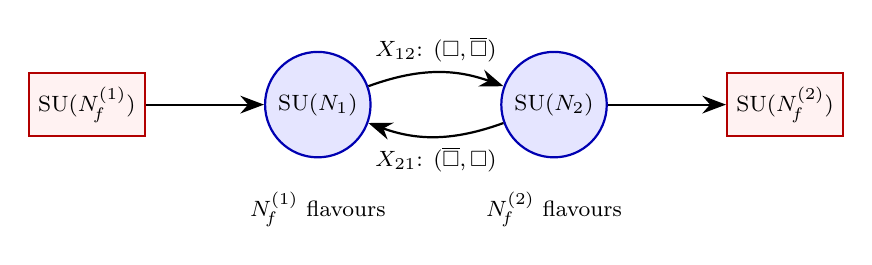
\begin{tikzpicture}[
  node distance=3cm,
  gauge/.style={circle, draw=blue!70!black, thick,
    fill=blue!10, minimum size=1.2cm, font=\footnotesize},
  arrow/.style={-{Stealth[length=3mm]}, thick}
]
  \node[gauge] (A) {$\SU{N_1}$};
  \node[gauge, right of=A] (B) {$\SU{N_2}$};

  \draw[arrow, bend left=20] (A) to node[above, font=\footnotesize]
    {$X_{12}$: $(\fund, \antifund)$} (B);
  \draw[arrow, bend left=20] (B) to node[below, font=\footnotesize]
    {$X_{21}$: $(\antifund, \fund)$} (A);

  \node[below=0.3cm of A, font=\footnotesize] {$\Nf^{(1)}$ flavours};
  \node[below=0.3cm of B, font=\footnotesize] {$\Nf^{(2)}$ flavours};

  % External flavours as squares
  \node[rectangle, draw=red!70!black, thick, fill=red!5,
    minimum size=0.8cm, font=\footnotesize,
    left=1.5cm of A] (F1) {$\SU{\Nf^{(1)}}$};
  \node[rectangle, draw=red!70!black, thick, fill=red!5,
    minimum size=0.8cm, font=\footnotesize,
    right=1.5cm of B] (F2) {$\SU{\Nf^{(2)}}$};

  \draw[arrow] (F1) -- (A);
  \draw[arrow] (B) -- (F2);
\end{tikzpicture}
\end{center}

In this quiver, circular nodes represent gauge groups (dynamical)
and square nodes represent global flavour symmetries (spectator).

\subsection{Seiberg duality as quiver mutation}

Seiberg duality can be applied to \emph{one node at a time} in a
quiver gauge theory~\cite{IS9506084}.  The procedure is called
\textbf{quiver mutation}:
\begin{enumerate}
  \item Choose a node with gauge group $\SU{\Nc}$.
  \item Count the total number of \emph{effective flavours}
    $\Nf^{\text{eff}}$ at that node: this includes both the external
    flavours and the bifundamentals from adjacent nodes.
  \item Replace the node by $\SU{\Nf^{\text{eff}} - \Nc}$, add
    the appropriate meson fields (composites of the original
    bifundamentals passing through the dualised node), and modify the
    superpotential according to the standard Seiberg duality map.
\end{enumerate}

The mutation rule preserves all 't~Hooft anomaly coefficients and
maps the moduli space correctly.  Successive mutations at different
nodes generate a \emph{duality web} of physically equivalent
descriptions of the same IR physics.

\subsection{Product group dualities}

Intriligator and Seiberg~\cite{IS9506084} extended the duality
programme to product gauge groups, finding dualities and
\emph{trialities} (three equivalent descriptions) for specific
product group theories.  The key insight is that Seiberg duality is
\emph{local}: it acts on one gauge group factor at a time, treating
the other factors as global symmetries from the perspective of the
dualised node.

For the dualised Standard Model, the product group structure
$\SU{3}_C \times \SU{2}_L \times \UU{1}_Y$ (or its Pati--Salam
extension $\SU{4} \times \SU{2}_L \times \SU{2}_R$) is naturally
embedded in a quiver.  The duality acts on the colour factor
$\SU{3}_C$ (or $\SU{4}$), treating the electroweak factors as
spectator global symmetries.


%% ========================================================================
%%  SECTION 7: The Duality Cascade
%% ========================================================================
\section{The Duality Cascade}
\label{sec:cascade}

A remarkable application of Seiberg duality to product gauge groups
is the \textbf{duality cascade} of Klebanov and
Strassler~\cite{KlebanovStrassler2000}.

\subsection{Setup}

Consider the gauge theory $\SU{N+M} \times \SU{N}$ with
bifundamental chiral superfields $A_1, A_2$ in the
$(\fund, \antifund)$ and $B_1, B_2$ in the $(\antifund, \fund)$,
together with a quartic superpotential:
\[
  W = h\,\epsilon^{ij}\epsilon^{kl}\,
  \Tr(A_i B_k A_j B_l)\,.
\]

This theory arises from $N$ regular and $M$ fractional D3-branes
placed at the tip of a conifold singularity in type IIB string
theory, but the field theory can be analysed independently.

\subsection{The cascade mechanism}

When $M > 0$, the $\SU{N+M}$ factor has more colours than the
$\SU{N}$ factor.  As the theory flows to the IR:
\begin{enumerate}
  \item The $\SU{N+M}$ factor becomes more strongly coupled.
    Applying Seiberg duality to the $\SU{N+M}$ node:
    \[
      \SU{N+M} \times \SU{N}
      \;\xrightarrow{\;\text{dualise}\;}
      \;\SU{N-M} \times \SU{N}\,.
    \]
    (The effective number of flavours at the $\SU{N+M}$ node is
    $2N$ from the bifundamentals, giving a dual gauge group
    $\SU{2N - (N+M)} = \SU{N-M}$.)
  \item After the duality, the $\SU{N}$ factor now has more
    colours.  Dualising it next gives
    $\SU{N-M} \times \SU{N-2M}$.
  \item The process repeats, \emph{cascading}:
    \[
      \SU{N+M} \times \SU{N}
      \to \SU{N-M} \times \SU{N}
      \to \SU{N-M} \times \SU{N-2M}
      \to \cdots
    \]
    Each step reduces the effective rank by~$M$.
\end{enumerate}

\subsection{The endpoint}

After approximately $N/M$ steps, the cascade terminates when one
gauge group factor reaches $\SU{M}$.  The final theory is
$\SU{2M} \times \SU{M}$, which confines.  The IR physics exhibits
\textbf{chiral symmetry breaking} and a mass gap, analogous to
QCD confinement.

The cascade provides a concrete mechanism by which a theory that is
UV-free (or conformal) at high energies flows through a sequence of
Seiberg dualities to a confining theory at low energies.
In the string theory realisation, the cascade corresponds to the
radial evolution along a warped deformed conifold geometry, where
the decreasing five-form flux corresponds to the decreasing rank of
the gauge group.

\begin{remark}[Beyond these lectures]
The geometric interpretation of the duality cascade requires the
framework of the AdS/CFT correspondence, which lies beyond the scope
of these lectures.  We refer to the original
paper~\cite{KlebanovStrassler2000} and the review
by Strassler~\cite{Strassler2005} for the complete treatment.
\end{remark}


%% ========================================================================
%%  SECTION 8: Synthesis
%% ========================================================================
\section{Synthesis: The Duality Landscape and the Dualised SM}
\label{sec:synthesis}

\subsection{Master comparison table}

We collect the dualities surveyed in this lecture and in Lecture~3
into a single comparison table.

\renewcommand{\arraystretch}{1.5}
\begin{table}[h!]
\centering
\small
\begin{tabular}{@{}p{2.0cm} p{2.3cm} p{2.3cm} p{2.0cm} p{2.3cm} p{2.5cm}@{}}
\toprule
\textbf{Duality} &
\textbf{Electric} &
\textbf{Magnetic} &
\textbf{Mesons} &
\textbf{Conf.\ Window} &
\textbf{Key Feature} \\
\midrule
\textbf{Seiberg} (Lec.~3) &
$\SU{\Nc}$, $\Nf\!\times\!(\fund,\antifund)$ &
$\SU{\Nf\!-\!\Nc}$ &
$M = Q\widetilde{Q}$ (sym.\ matrix) &
$\frac{3\Nc}{2} < \Nf < 3\Nc$ &
Prototype \\
\midrule
\textbf{KS} (\S\ref{sec:kutasov-schwimmer}) &
$\SU{\Nc}$, $\Nf\!+\!\adj$, $W\!=\!\Tr\Phi^{k+1}$ &
$\SU{k\Nf\!-\!\Nc}$ &
$M_j = Q\Phi^j\widetilde{Q}$, $j=0,\ldots,k\!-\!1$ &
$\frac{3\Nc}{k+1} < \Nf < \frac{3\Nc}{k}$ &
$k\!=\!1$ recovers Seiberg \\
\midrule
\textbf{SO} (\S\ref{sec:SO-duality}) &
$\SO{\Nc}$, $\Nf$ vectors &
$\SO{\Nf\!-\!\Nc\!+\!4}$ &
$M_{ij}=Q_iQ_j$ (symmetric) &
$\frac{3(\Nc\!-\!2)}{2} < \Nf < 3(\Nc\!-\!2)$ &
Shift $+4$ \\
\midrule
\textbf{Sp} (\S\ref{sec:Sp-duality}) &
$\Sp{\Nc}$, $2\Nf$ fund. &
$\Sp{\Nf\!-\!\Nc\!-\!2}$ &
$M_{ij}=Q_iJQ_j$ (antisym.) &
$\frac{3(\Nc\!+\!1)}{2} < \Nf < 3(\Nc\!+\!1)$ &
Shift $-2$ \\
\midrule
\textbf{s-confining} (\S\ref{sec:s-confinement}) &
Various (Table~\ref{tab:s-confining}) &
\textit{none} (trivial) &
All composites &
\textit{boundary} &
No dual gauge group \\
\midrule
\textbf{Cascade} (\S\ref{sec:cascade}) &
$\SU{N\!+\!M}\!\times\!\SU{N}$, bifundamentals &
$\SU{N\!-\!M}\!\times\!\SU{N}$ (iterates) &
Generated at each step &
\textit{flows} &
RG cascade \\
\bottomrule
\end{tabular}
\caption{Master comparison table of $\mathcal{N}=1$ SUSY dualities.
The conformal window column gives the range of $\Nf$ for which both
the electric and magnetic theories are asymptotically free and flow to
the same interacting fixed point.  The ``shift'' in the SO and Sp
rows refers to the difference in the dual gauge group rank relative
to the SU case: $\SU{\Nf - \Nc + 0}$ vs.\ $\SO{\Nf - \Nc + 4}$
vs.\ $\Sp{\Nf - \Nc - 2}$.}
\label{tab:master-comparison}
\end{table}

\subsection{Unifying thread: anomaly matching}

Across the entire landscape, the unifying consistency check is
\textbf{'t~Hooft anomaly matching}.  In every case --- SU, SO, Sp,
product groups, KS --- the anomaly coefficients of the global
symmetry group match exactly between the electric and magnetic
descriptions, as polynomial identities in $\Nc$ and $\Nf$.

We have verified this explicitly:
\begin{itemize}
  \item $\SU{\Nc}$ (Seiberg): six independent anomaly coefficients
    matched in Lecture~3.
  \item $\SO{\Nc}$: $\SU{\Nf}^2\,\UU{1}_R$ anomaly matched in
    \S\ref{ssec:SO-anomaly}.
  \item $\Sp{\Nc}$: $\SU{2\Nf}^2\,\UU{1}_R$ anomaly matched in
    \S\ref{ssec:Sp-anomaly}.
\end{itemize}

Each of these is an \emph{exact} statement, valid for all values of
$\Nc$ and $\Nf$ within the duality range.  This universality of
anomaly matching provides strong evidence that electric--magnetic
duality is a deep structural feature of strongly coupled gauge
theories, not a coincidence of specific group-theoretic numerology.

\subsection{Relevance to the dualised SM}

Which of these dualities is most relevant to the dualised Standard
Model programme of Lectures~7--8~\cite{CacciapagliaSannino2024}?

\begin{enumerate}
  \item \textbf{Kutasov--Schwimmer duality with adjoint matter}
    is the most directly relevant.  The dualised SM embeds the SM
    gauge group in a Pati--Salam-type structure $\SU{4} \times
    \SU{2}_L \times \SU{2}_R$, where the $\SU{4}$ factor carries
    both fundamental quarks and potentially adjoint matter from the
    breaking of a larger gauge group.  The KS duality with $k=1$
    (recovering standard Seiberg duality after integrating out the
    adjoint) provides the natural UV framework.

  \item \textbf{Product group dualities} are relevant because the SM
    has a product gauge group structure.  The quiver mutation
    technique shows that duality can be applied node-by-node: one can
    dualise the colour $\SU{3}_C$ factor while leaving the
    electroweak factors as spectators.

  \item \textbf{The SO and Sp dualities} demonstrate the robustness
    of the duality phenomenon.  While the SM gauge group involves
    SU-type factors (not SO or Sp), the existence of dualities for
    all classical Lie groups suggests that the mechanism is deeply
    structural.

  \item \textbf{s-Confinement} is relevant to the QCD-like
    sector.  If the electric theory has a number of flavours near the
    s-confining boundary, the confined degrees of freedom
    (composites) naturally map to the physical hadrons.
\end{enumerate}

The central lesson of this lecture is that \textbf{duality is not a
special trick for one particular gauge group}: it is a pervasive
structural feature of strongly coupled $\mathcal{N}=1$ gauge theories.
The dualised Standard Model sits within this landscape, drawing on
the specific features of $\SU{N}$ duality with fundamental (and
potentially adjoint) matter.

\begin{previewbox}[title={Preview: Lecture 10}]
  In Lecture~10, we will connect the abstract meson matrix~$M^i{}_j$
  of Seiberg duality to the physical meson spectrum of QCD.  The
  question: if the SM quarks are ``dual quarks'' in a magnetic
  description, what are the corresponding mesons $M = Q\widetilde{Q}$,
  and how do they relate to the observed $\pi$, $K$, $D$, $B$
  mesons?  This requires confronting the transition from the SUSY
  duality landscape to the non-supersymmetric real world --- the
  central challenge of the dualised SM programme.
\end{previewbox}


%% ========================================================================
%%  SUMMARY
%% ========================================================================
\section{Summary}
\label{sec:summary-L9}

In this lecture we have:
\begin{enumerate}
  \item Presented the \textbf{Kutasov--Schwimmer duality} for
    $\SU{\Nc}$ with $\Nf$ flavours and an adjoint $\Phi$ with
    $W = \Tr(\Phi^{k+1})/(k+1)$: the dual is $\SU{k\Nf - \Nc}$
    with $k$ meson species $M_j = Q\Phi^j\widetilde{Q}$.
  \item Verified the crucial \textbf{$k=1$ limit}: integrating out
    the massive adjoint recovers standard Seiberg duality for
    $\SU{\Nf - \Nc}$.
  \item Established the \textbf{$\SO{\Nc}$ duality} with dual gauge
    group $\SO{\Nf - \Nc + 4}$ and verified the
    $\SU{\Nf}^2\,\UU{1}_R$ anomaly matching.
  \item Established the \textbf{$\Sp{\Nc}$ duality} with dual gauge
    group $\Sp{\Nf - \Nc - 2}$ and verified the
    $\SU{2\Nf}^2\,\UU{1}_R$ anomaly matching.
  \item Classified \textbf{s-confining theories} following
    Cs\'aki--Schmaltz--Skiba, identifying them as the boundary
    cases where the magnetic gauge group rank vanishes.
  \item Described \textbf{product group dualities} (quiver mutation)
    and the \textbf{Klebanov--Strassler duality cascade}.
  \item Synthesised the landscape into a
    \textbf{master comparison table} (Table~\ref{tab:master-comparison})
    and identified the Kutasov--Schwimmer duality with adjoint matter
    as most relevant to the dualised SM programme.
\end{enumerate}


%% ========================================================================
%%  BIBLIOGRAPHY
%% ========================================================================
\begin{thebibliography}{99}

\bibitem{Seiberg1995}
  N.~Seiberg,
  ``Electric--magnetic duality in supersymmetric non-Abelian gauge
  theories,''
  \textit{Nucl.\ Phys.} \textbf{B435} (1995) 129
  [\texttt{hep-th/9411149}].

\bibitem{KS9505004}
  D.~Kutasov and A.~Schwimmer,
  ``On duality in supersymmetric Yang--Mills theory,''
  \textit{Phys.\ Lett.} \textbf{B354} (1995) 315
  [\texttt{hep-th/9505004}].

\bibitem{KSS9507040}
  D.~Kutasov, A.~Schwimmer, and N.~Seiberg,
  ``Chiral rings, singularity theory and electric--magnetic duality,''
  \textit{Nucl.\ Phys.} \textbf{B459} (1996) 455
  [\texttt{hep-th/9507040}].

\bibitem{IS9506101}
  K.~Intriligator and N.~Seiberg,
  ``Duality, monopoles, dyons, confinement and oblique confinement
  in supersymmetric $\mathrm{SO}(N_c)$ gauge theories,''
  \textit{Nucl.\ Phys.} \textbf{B444} (1995) 125
  [\texttt{hep-th/9506101}].

\bibitem{IS1995}
  K.~Intriligator and N.~Seiberg,
  ``Lectures on supersymmetric gauge theories and electric--magnetic
  duality,''
  \textit{Nucl.\ Phys.\ Proc.\ Suppl.} \textbf{45BC} (1996) 1
  [\texttt{hep-th/9509066}].

\bibitem{IS9506084}
  K.~Intriligator and N.~Seiberg,
  ``Phases of $\mathcal{N}=1$ theories in two dimensions,''
  \textit{Nucl.\ Phys.} \textbf{B431} (1994) 551
  [\texttt{hep-th/9506084}].

\bibitem{CSS9612207}
  C.~Cs\'aki, M.~Schmaltz, and W.~Skiba,
  ``A systematic approach to confinement in $\mathcal{N}=1$
  supersymmetric gauge theories,''
  \textit{Phys.\ Rev.\ Lett.} \textbf{78} (1997) 799
  [\texttt{hep-th/9612207}].

\bibitem{KlebanovStrassler2000}
  I.~R.~Klebanov and M.~J.~Strassler,
  ``Supergravity and a confining gauge theory: duality cascades
  and $\chi$SB-resolution of naked singularities,''
  \textit{JHEP} \textbf{0008} (2000) 052
  [\texttt{hep-th/0007191}].

\bibitem{Strassler2005}
  M.~J.~Strassler,
  ``The duality cascade,''
  [\texttt{hep-th/0505153}].

\bibitem{Peskin1997}
  M.~E.~Peskin,
  ``Duality in supersymmetric Yang--Mills theory,''
  [\texttt{hep-th/9702094}].

\bibitem{CacciapagliaSannino2024}
  G.~Cacciapaglia and F.~Sannino,
  ``The Dualised Standard Model,''
  [\texttt{arXiv:2407.17281}].

\end{thebibliography}

\end{document}
